\chapter{Background}
The biologist Carl Woese 2009 suggested that “Organisms are resilient patterns in a turbulent flow—patterns in an energy flow” \cite{Woese}. If this somewhat captures life, then the formation and maintenance of patterns are essential. On the sub-cellular level, an important component conferring structure and organization is the cytoskeleton. The cytoskeleton is a complex, dynamic network of protein filaments which can be found in the cytoplasm of all cells, including bacteria and archaea. Eukaryotes employ three different types of filaments: microtubules, actin filaments and intermediate filaments. These filaments interact interact with a plethora of other biopolymers in the cell, allowing the cytoskeleton to fulfill vital functions in a diverse set of domains, such as locomotion of the cell, maintaining structural integrity, chromosome segregation and cytokinesis during mitosis and the transport of cargoes within the cell. The cytoskeleton confers structure to the cell, but what confers structure to the cytoskeleton itself? While some of the patterning stems from interactions with other large entities, such as the cell membrane, the organization of the cytoskeleton partly emerges from the collective behavior of the involved cytoskeletal polymers. In other words, the cytoskeleton and its associates are known to display self-organization \parencite{Karsenti2008}. This work aims to expand our understanding of how, and to which extent, cytoskeletal polymers interact to give rise to supramolecular patterning. \par
To minimize the number of factors which could possibly give rise to patterns such to reveal underlying molecular mechanisms, we followed a bottom-up approach, where we sought to reconstitute cytoskeletal features \textit{in-vitro} with a minimum number of components. We focused on microtubules, where we were interested in two cytoskeletal systems of which they are prominent members: (1) Axonal microtubule arrays. (2) Mitotic spindle? These two systems are very different, which is also reflected by the different behavior of microtubules within them. Thus, this thesis contains two parts, each dedicated to one of these systems. As in both systems, microtubules are an integral part of the experimental setup, I here offer an introduction to them. I here also give a brief introduction to the microtubule-associated proteins explored in the experiments.
\section{Microtubules}
The most obvious characteristic of microtubules is their very high persistence length in the low millimeter range \parencite{Portran2013}, which allows them to stretch over distances comparable to the size of a whole cell. The microtubule lattice can be described as a lateral association of so-called protofilaments, which are linear strands of $\alpha$- and $\beta$-tubulin heterodimers (\autoref{MTintro}A). This leads to the cylindrical structure of microtubules with an outer diameter of 25 nm (\autoref{MTintro}B), a feature allowing for their high persistence length. Only at high concentrations of free tubulin spontaneous nucleation can occur \parencite{Fygenson1994}, which gives the cell the ability to fine-tune the number of microtubules over time and space: The \textit{de novo} assembly of microtubules is directed by designated $\gamma$-tubulin \textit{nucleation} complexes prominent in microtubule-organizing centers (MTOCs) and also along pre-existing microtubules \parencite{Guttinger2009, Janson2007}.

\subsection{Tubulin}
Tubulin is an eukaryotic protein highly conserved throughout evolution. In cells, tubulin exists almost exclusively as the $\alpha\beta$-tubulin heterodimer. $\alpha$- and $\beta$-tubulin are conserved throughout eukaryotes, sharing over 40\% sequence identity with nearly the same secondary and tertiary structures \parencite{DOWNING199816}. Each tubulin monomer is a globular protein and consists of three closely interacting domains: an N-terminal nucleotide-binding domain, an intermediate domain, and a carboxy-terminal (C-terminal) helical region \parencite{ALUSHIN20141117}. The disordered, negatively charged C-terminal tails of tubulin protrude outwards from the microtubule surface. As is the case with many other proteins, tubulins express in different isoforms and can be modulated by post-translational modifications, thus providing an additional level of microtubule regulation \parencite{Janke2014}. Modification of the C-terminal region in particular has been found to affect microtubule properties and their interactions with other proteins \parencite{Janke2020}. 

\subsection{Dynamic instability}
Owing to the uniform orientation of the tubulin dimers, microtubules are directional polymers,  with the $\beta$-subunits pointing to one end (called ‘plus end’) and the $\alpha$-subunits pointing to the opposite end (called ‘minus end’). \textit{In vivo}, minus ends never polymerize, and microtubule growth happens exclusively at the plus end \parencite{Dammermann2003R614}. In spite of their high stiffness, microtubules are no static structures, instead their plus ends are stochastically switching between phases of growth and hrinkage. This property is termed \textit{dynamic instability}. It stems from the existence of two conformationally distinct populations of tubulin dimers: GTP-tubulin and GDP-tubulin, having GTP respectively GDP bound to their $\beta$-tubulin. Mostly, GTP-tubulin add to the lattice. Once incorporated, the $\beta$-tubulin quickly hydrolyzes its GTP, which for an unbound dimer would result in a curved conformation. Within the microtubule body though, this curvature cannot be realized due to the interaction with neighboring dimers, giving rise to an initial tension within the lattice. Hence, GTP-hydrolysis has no immediate consequences, unless it occurs at an microtubule end: There, GDP-tubulin have more degrees of freedom and can relax to their bent state, thereby releasing energy. This energy in turn can be used to break bonds, enabling more GDP-tubulin to relax. Shrinkage occurs if this depolymerization propagates on: A \textit{catastrophe} event is given. As depicted in \autoref{MTintro}C, entire protofilaments curl up along the microtubule. Thus, for a microtubule to grow, a certain fraction of GTP-tubulin has to cap its ends. A regain of this cap during shrinkage is termed a rescue event, which initiates a new period of growth. \parencite{Janosi2002}

\begin{figure}[h!tb]
\centering
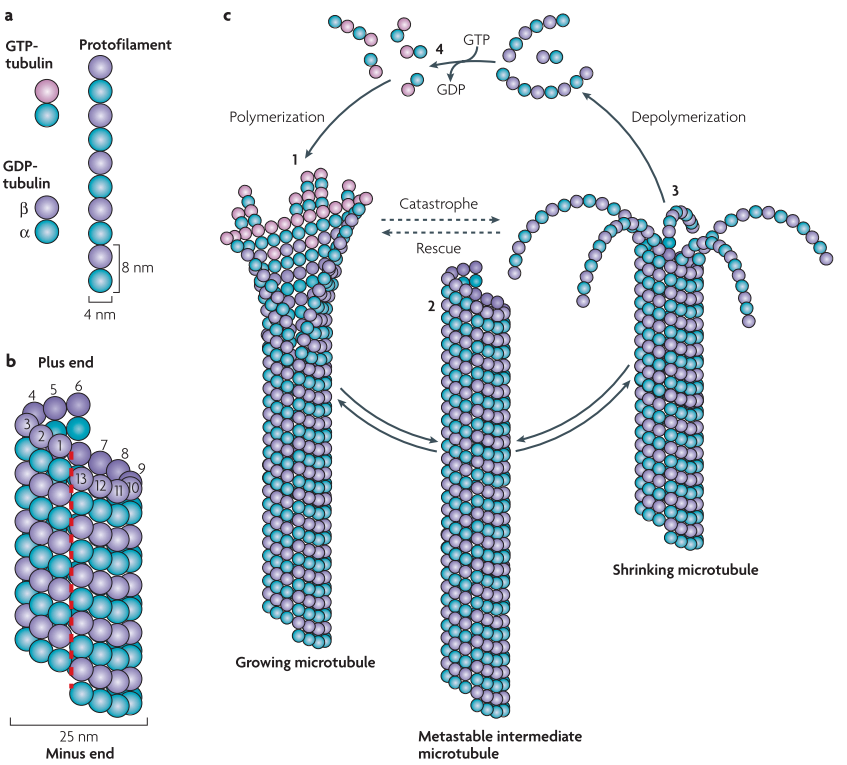
\includegraphics[scale=0.65]{Figures/MTintro.png}
\caption[Introduction to microtubules.]{
(A) Microtubules consist of $\alpha\beta$ heterodimers. While $\alpha$-tubulin normally retains its GTP, the GTP molecule of $\beta$-tubulin can be both hydrolyzed and exchanged for ADP. (B) \textit{In vivo}, microtubules are composed of 13 protofilaments. Since the \SI{12}{\nm} helical pitch does not equal the dimer length, a lattice seam occurs. (C) Due to the GTP-hydrolysis of incorporated $\beta$-tubulin, microtubule ends undergo a permanent cycle of growth (1) and shrinkage (3), closed by the exchange of GDP for GTP for the disassembly products (4). This cycle can briefly come to a halt during a less prevalent metastable state (2), from which microtubules can switch either to growth or to shrinkage. All sketches adapted from \cite{Akhmanova2008}.
	}\label{MTintro}
\end{figure}
 \FloatBarrier

\section{Microtubule-associated proteins}
The vast functional diversity of microtubules is enabled by their interactions with microtubule-associated proteins (MAPs). \cite{BODAKUNTLA2019804} categorize MAPs into different groups depending on their mode of action, namely i) molecular motors
generating movement along microtubules, ii) enzymes destabilizing the microtubule lattice, iii) MAPs promoting microtubule nucleation, iv) microtubule-end binding proteins and v) structural MAPs controlling microtubule polymerization, stabilization and assembly into microtubule bundles. One MAP may belong to several of these groups, for instance, the molecular motor Kip3 is known to also cause microtubule polymerization \parencite{Gardner2011a}. In the following, an introduction is given to the MAPs which I worked with in the context of this thesis.

\subsection{Ase1}
Ase1 (a member of the Ase1/PRC1/Map65 family) is a microtubule crosslinker known to organize microtubule arrays during mitosis as well as interphase in the fission yeast S. pombe \parencite{Loiodice2005} (\autoref{Ase1}A). The geometry of Ase1/MAP65/PRC1 MT binding sites favors antiparallel MT, which results in increased Ase1/MAP65/PRC1 affinities for antiparallel MT overlaps and preferential antiparallel crosslinking activity 6–11. During mitosis, Ase1/MAP65/PRC1 proteins are found preferentially at the spindle midzone, and are involved in spindle integrity and regulation of spindle elongation 4,5,8. Fission yeast, S. pombe, Ase1 deletion mutants, although viable, exhibit interphase MTs with reduced bundling and mitotic spindles that often fall apart as they elongate in anaphase 4,5. The preferred binding of Ase1/MAP65/PRC1 family proteins to antiparallel MTs leads to the recruitment of other proteins at the midzone that can locally alter MT dynamics, such as CLASP 12–14 or kinesin-4 (Bieling, Telley and Surrey, 2010; Mani et al. 2021). By recruiting these additional factors, Ase1 family proteins can differentially regulate the dynamics of bundled MTs, specifically affecting the dynamics of antiparallel bundles 7,15. Additionally, Ase1 family members themselves are also known to have direct effects on MT dynamics. In vitro experiments have shown that MAP65-1, upon crosslinking MTs, promotes rescues 16. Based on the modeling of their observed overlap dynamics, Stoppin-Mellet et al. predicted MAP65-1 to have more effect on antiparallel MTs compared to parallel ones. \par
Ase1 possesses a structured N-terminal domain, a central spectrin domain, and an intrinsically disordered C-terminal domain \parencite{Kapitein2008,Kellogg2018}. The N-terminal domain supports homodimerization of Ase1 and is necessary for microtubule crosslinking activity \parencite{Janson2007}. The spectrin domain and the unstructured C-terminal interact with the microtubule \parencite{Kellogg2018}. Ase1 interacts with microtubules diffusively by exhibiting a one-dimensional random walk along the microtubule lattice. When diffusing on a single microtubule, the free microtubule-binding domain samples a large space, allowing for "catching" of another microtubule which subsequently is crosslinked to the first microtubule, preferably in antiparallel fashion (\cite{Janson2007}, \autoref{Ase1}B). Within the resulting antiparallel microtubule bundle, Ase1 does still diffuse, albeit with an approximately eight-times lower diffusion coefficient than on single microtubules \parencite{lanskydiffusible2015}.
\begin{figure}[h!tb]
\centering
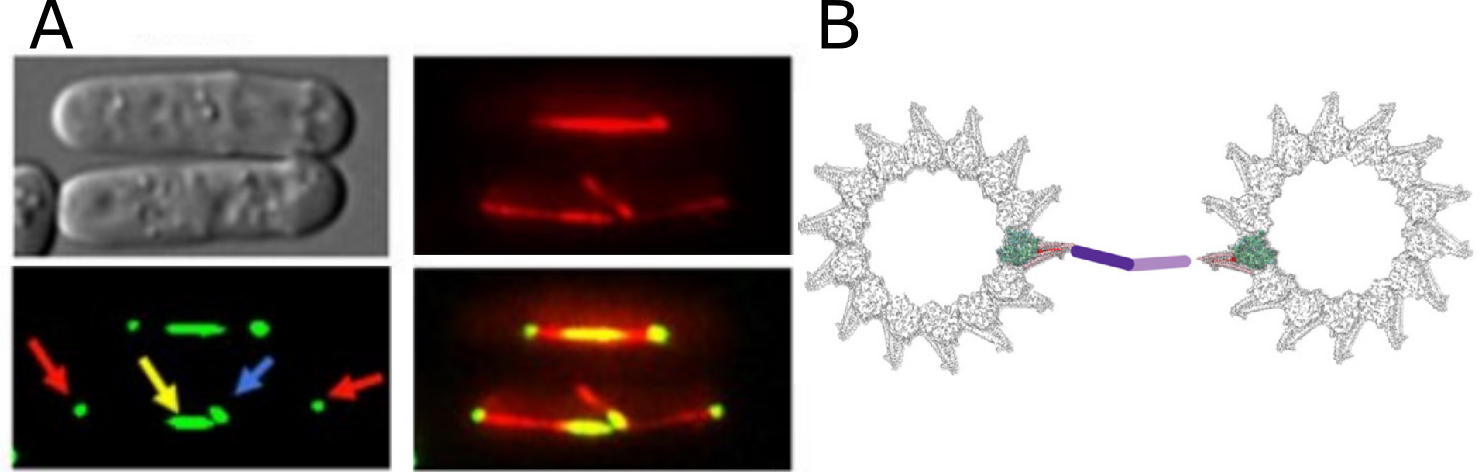
\includegraphics[scale=1.1]{Figures/Ase1.png}
\caption[Introduction to Ase1.]{
(A) 3D projection images of wild-type S. pombe cells taken during mitosis, with tubulin (CFP-tub1p) in red and Ase1 (Ase1-GFP) in green. Top-left picture taken with differential interference contrast (DIC) microscopy. The yellow arrow indicates the spindle midzone, where Ase1 is binding in between antiparallel microtubule overlaps. Adopted from \cite{Loiodice2005}. (B) A model of how PRC1, a Ase1 homologue, binds to two antiparallely aligned microtubules, based on cryo-EM data. The cryo-EM reconstruction is overlayed with shades of green and blue ($\alpha$ and $\beta$-tubulin) and pink (the microtubule-binding domains of PRC1). The dimerization domains of PRC1 are shown as cartoons in shades of purple (the cryo-EM study was conducted with a PRC1 construct without the dimerization domain). Adopted from \cite{Kellogg2016}. 
	}\label{Ase1}
\end{figure}

\subsection{Tau}
Tau is an intrinsically disordered protein mainly found in neuronal axons. Tau is involved in a number of neurodegenerative diseases (Gao et al., 2018; Iqbal et al., 2016; Morris et al., 2011), e.g., displacement of tau from the axon is one of the hallmark events during the onset of the Alzheimer’s disease (Zempel and Mandelkow, 2015). An important function of tau is to enhance the stability of microtubules, which it can influence directly \cite{Drechsel1992} as well as by its capability to regulate the interaction of other MAPs with the microtubule surface \parencite{Morris2011b}. For example, tau mislocalization leaves axonal microtubules unprotected against microtubule-severing enzymes, such as katanin (Qiang, 2006), which leads to their destabilization and the eventual degeneration of the axon. Tau can also regulate the microtubule interactions of other MAPs, such as molecular motors (Chaudhary et al., 2018; Dixit et al., 2008; Ebneth et al., 1998; Seitz et al., 2002; Trinczek et al., 1999; Vershinin et al., 2007). \par
As depicted in \autoref{tau}A, full-length adult tau is intrinsically disordered and includes a projection domain, a microtubule-binding region of four imperfect sequence repeats (R1-4), and a C-terminal domain \parencite{Himmler1381}.
Several different observations and explanations for how tau interacts with microtubules can be found in the literature \parencite{Morris2011b,Mcvicker2014,Kellogg2018}. For instance, it is known that tau can engage with microtubules in a mode where it diffuses along the microtubule (Hinrichs et al., 2012), and in another mode where it is stably bound to the microtubule \parencite{Mcvicker2014}. Recently, it was found that the tau microtubule binding repeats can bind to microtubules in a consistent, orderly fashion, enough so to allow for a high-resolution cryo-EM study (\autoref{tau}B-C) \parencite{Kellogg2018}. 
\begin{figure}[h!tb]
\centering
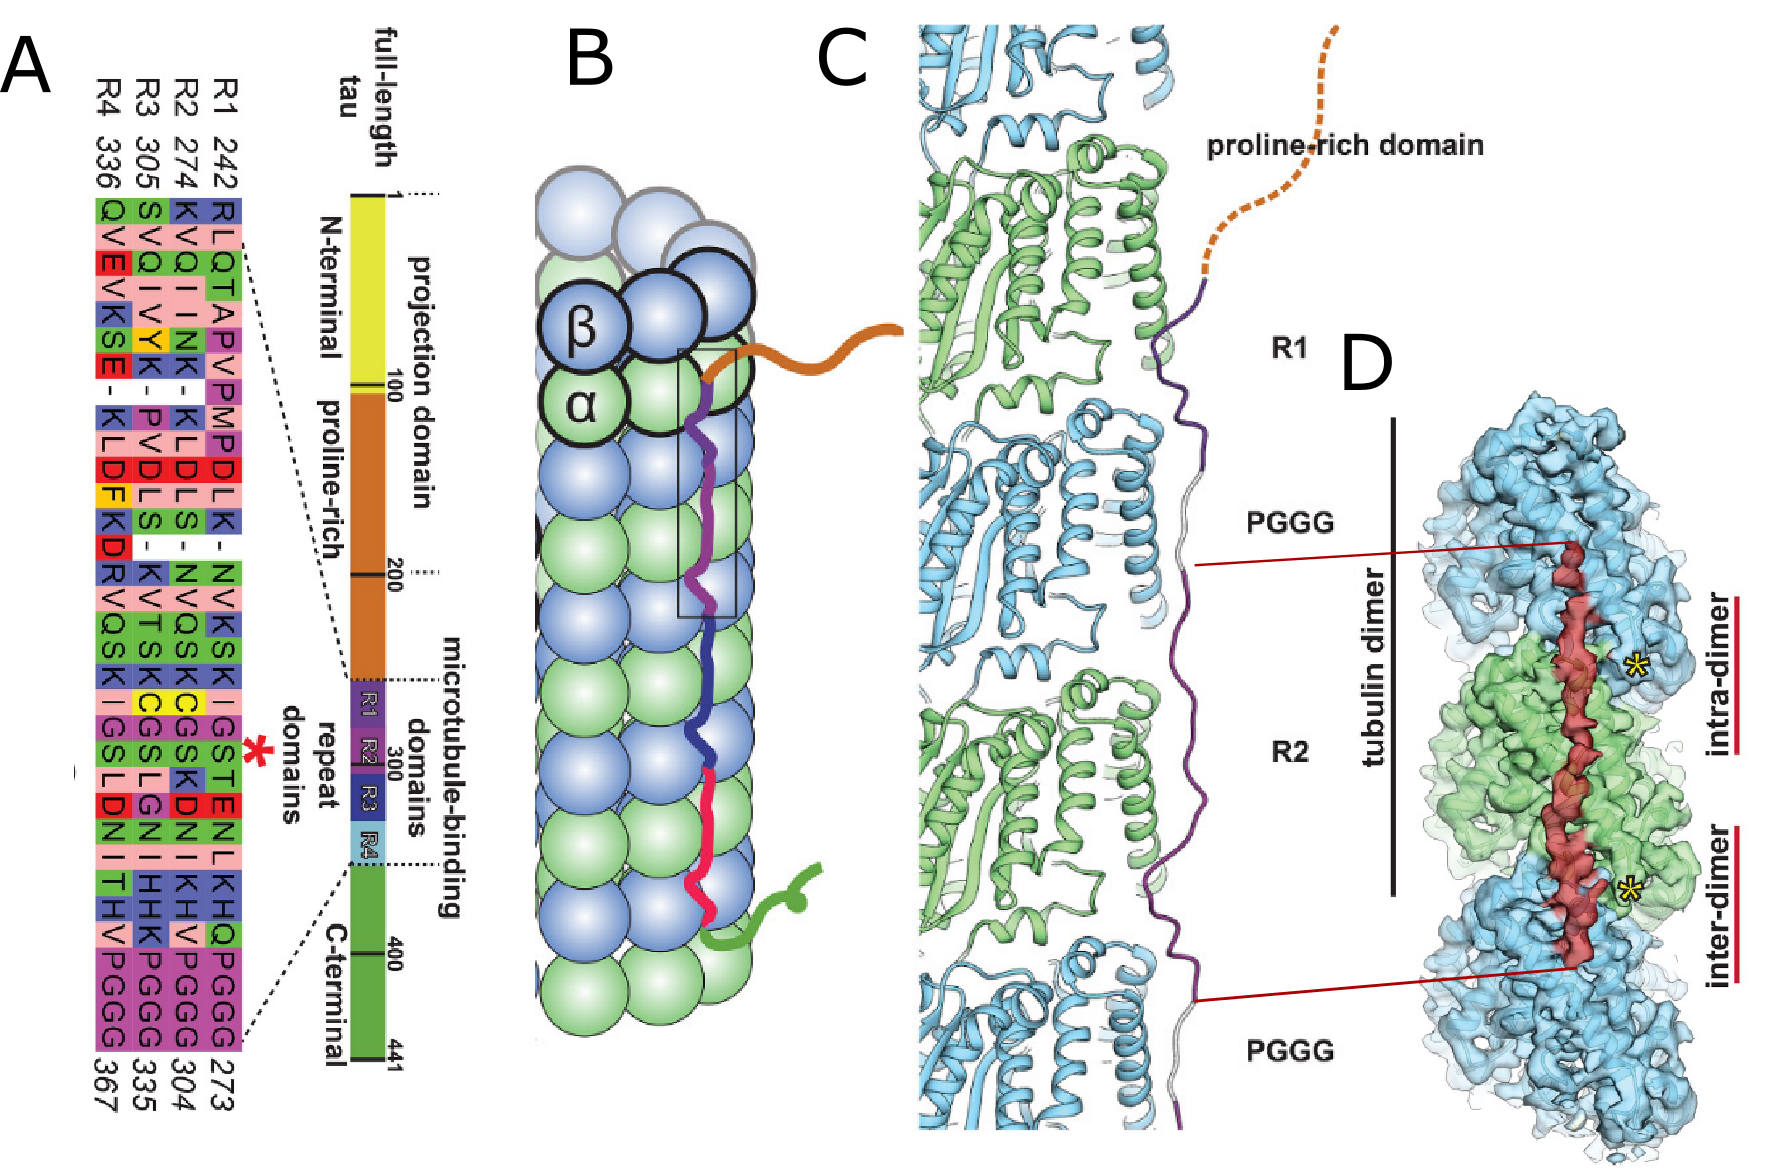
\includegraphics[scale=0.93]{Figures/tau.png}
\caption[Introduction to tau.]{
(A) Schematic of tau domain architecture. Inset shows the sequence alignment of the four repeat sequences, R1-4, that make up the repeat domain. (B) Model of full-length tau binding to microtubules and tubulin oligomers proposed by a recent cryo-EM study \parencite{Kellogg2018}. (C) Detailed representation of that model. (D) Cryo-EM density map of a part of the microtubule surface under the presence of tau, as observed by \cite{Kellogg2018} (top view, looking onto the surface of the microtubule). The additional density (in addition to tubulin) is colored in red and likely due to tau binding to the microtubule with its microtubule binding repeats. The PGGG sequences between the repeats were not visible on the density map, indicating that they did not bind to the microtubules in an orderly fashion. Adapted from \cite{Kellogg2018}. 
	}\label{tau}
\end{figure}

\subsection{Kinesin-1 and kinesin-8}
Molecular motors convert chemical energy in form of ATP into mechanical energy. One of the three large superfamilies of molecular motors are kinesins. To date more than 600 kinesin sequences with 45 kinesin genes in the human- 17 -genome \parencite{Endow3420} have been identified. Kinesins are divided into 14 kinesin sub-families based on their structure and function. We worked with two kinesins, namely kinesin-1 and Kip3 (a kinesin-8 family found in budding yeast). Both these kinesins move toward the microtubule plus-end along protofilaments, propelled by their motor domains (\autoref{kinesins}A). However, while kinesin-1 typically detaches from microtubules after a few hundred steps latest (each step being 8 nm long, the same as the inter-tubulin-dimer distance, see \cite{COY19993667}), Kip3 is much more processive, to a point where it usually reaches the plus end of the microtubule \cite{Varga2009}. This processivity is attributed to the tail domain of Kip3, which can bind to microtubules \parencite{SU2011751}. Kinesin-1 is known mainly for its function in transport of cargo along the microtubule \parencite{Endow3420}. Kip3 has the conspicuous characteristic of promoting microtubule depolymerization at the microtubule plus end, where they can accumulate (\autoref{kinesins}B). This causes Kip3 to differentially regulate microtubule length, as more Kip3 molecules land on longer microtubules, which therefore experience more depolymerization activity at their plus ends than short microtubules \parencite{Varga2009}.
\begin{figure}[h!tb]
\centering
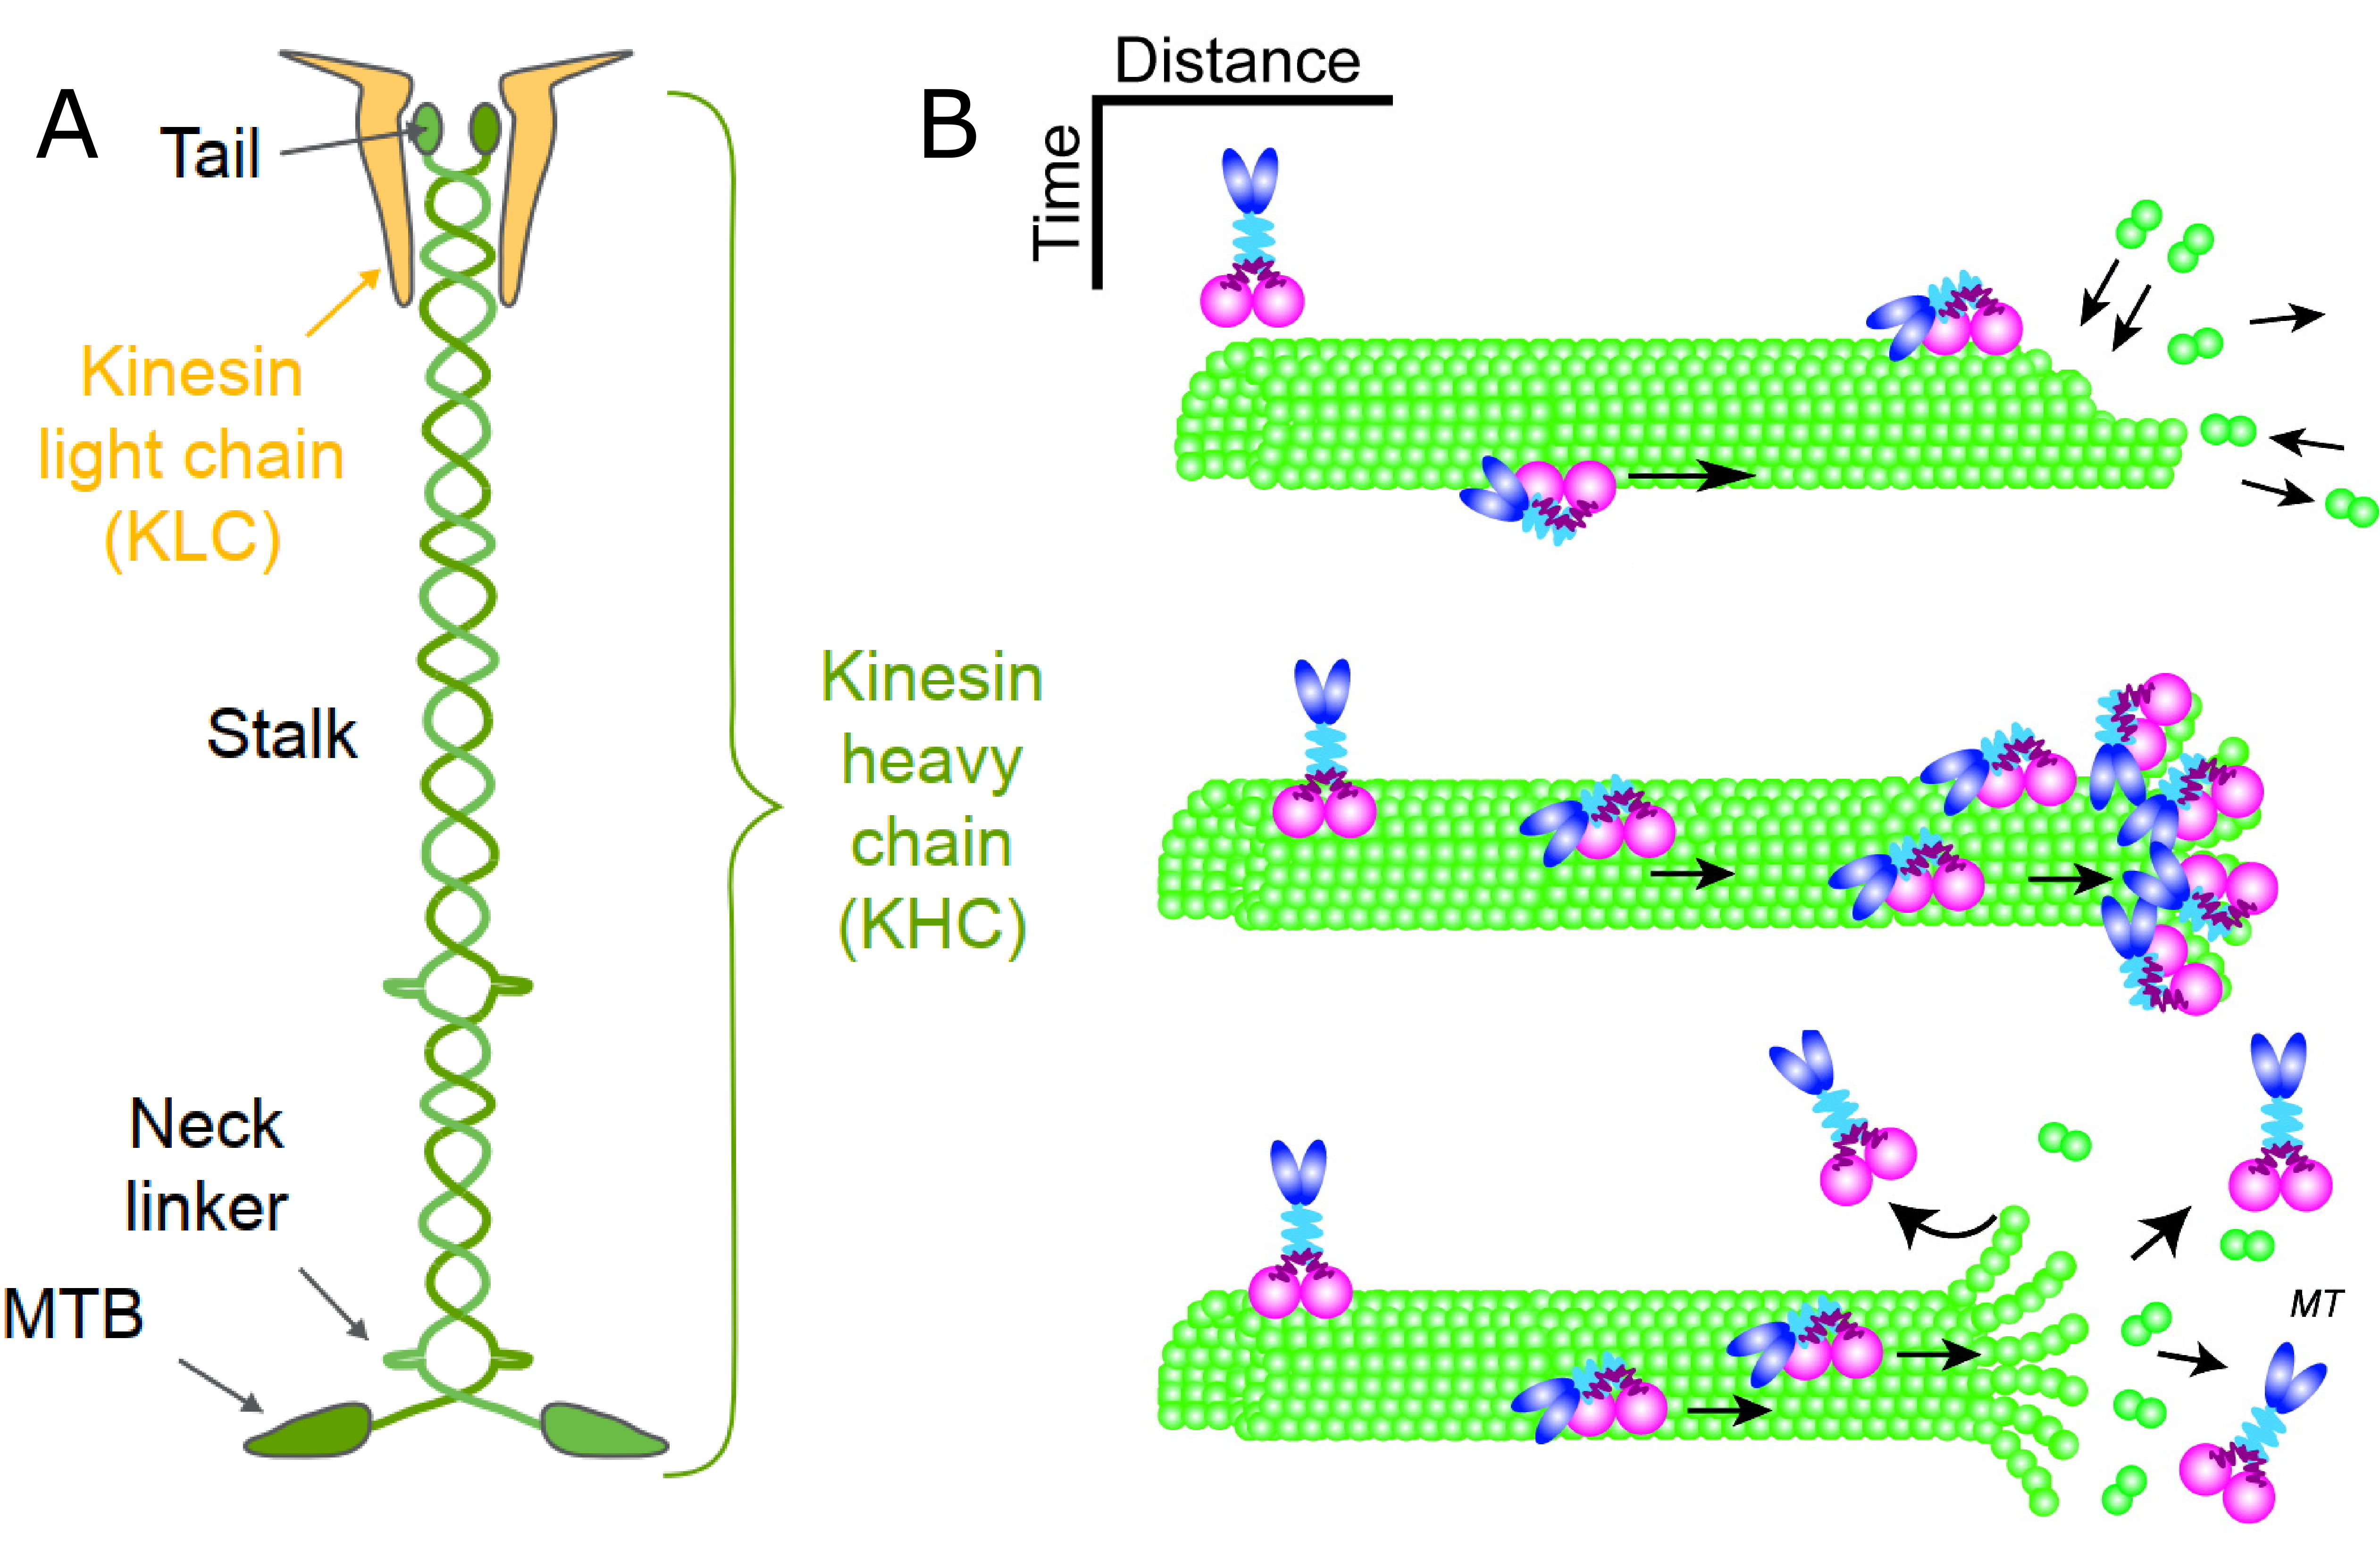
\includegraphics[scale=0.3]{Figures/kinesins.png}
\caption[Introduction to kinesins.]{
(A) Kinesin-1 is a heterotetrameric complex of two kinesin heavy chains (KHC) composed of a head, stalk and tail domain and two kinesin light chains (KLC). The motor domains alternately bind to the microtubule, where directed movement is generated by ATP hydrolysis. Adapted from \cite{kawaguchi}. (B) A model of Kip3 behavior on the microtubule. Over time, the number of Kip3 motors at the plus end of the MT increases. At the plus end, Kip3 motors stabilize a curved protofilament conformation until enough motors have accumulated to cause a catastrophe, initiating microtubule depolymerization. Adapted from \cite{weaver}.
	}\label{kinesins}
\end{figure}

\subsection{Katanin}
Katanin is a microtubule-severing enzyme, generating internal breaks in microtubules, thereby modulating their dynamics and organization \parencite{ROLLMECAK201096}. Katanin is composed of a catalytic (p60) and a regulatory (p80) subunit. The catalytic subunit contains the ATPase motor and is sufficient for microtubule severing \parencite{McNally2014}. The p80 subunit regulates binding to the centrosome and enhances microtubule binding \parencite{Joly3604}. ATP hydrolysis is required for severing activity, and the katanin p60 ATPase is stimulated by the microtubule19. By pulling on the C-terminal tails of tubulin, katanin achieves step-wise destabilization of local microtubule lattice contacts, ultimately leading to microtubule severing (\autoref{katanin}) \parencite{McNally2014}.
\label{sec:katanin}

\begin{figure}[h!tb]
\centering
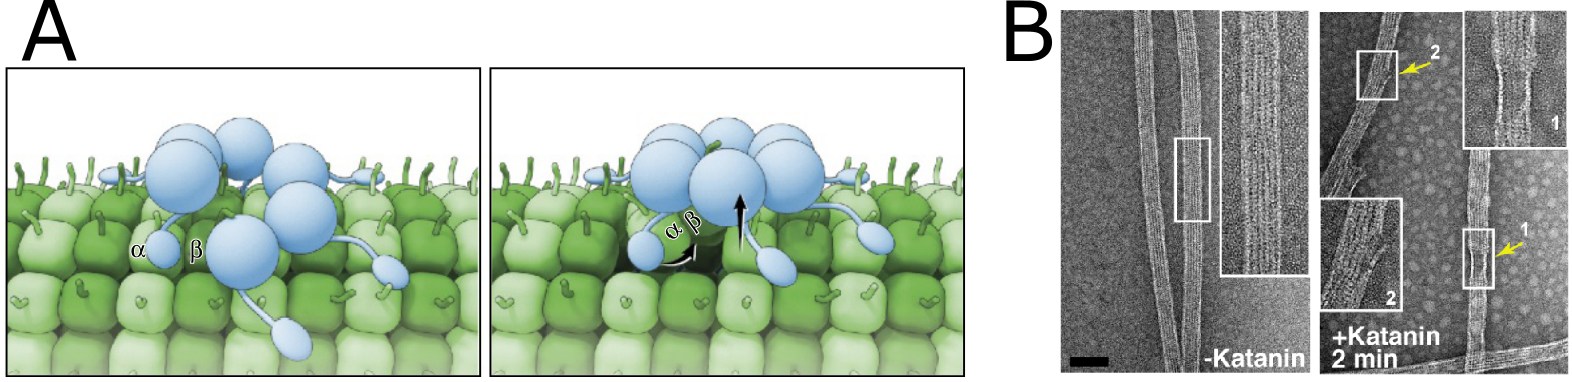
\includegraphics[scale=1.1]{Figures/katanin.png}
\caption[Introduction to katanin.]{
(A) Cartoon illustrating how katanin is hypothesized to extract tubulin dimers. Left, katanin (blue) assembles as a hexamer with each monomer's N-terminal domain emanating from the motor core and making multivalent interactions with the microtubule (green). The flexible tubulin C-terminal is engaged in the axial pore of the katanin hexamer. Right, ATP hydrolysis leads to closure of the ring that drags with it the bound C-terminal tail of a tubulin monomer. The cycle is repeated until lattice contacts unravel and the microtubule severs. Adapted from \cite{Zehr2017}. (B) GMPCPP-microtubules incubated with buffer or 100 nM katanin and visualized by transmission electron microscopy. Arrows indicate damage in the microtubule lattice. Adapted from \cite{Grigorieff2018}.
	}\label{katanin}
\end{figure}

\section{Employed microscopy methods}
\subsection{Total internal reflection (TIRF) microscopy}
The main experimental method employed during the course of this work was total internal reflection fluorescence (TIRF) microscopy. TIRF microscopy takes advantage of the physical phenomenon of total internal reflection, whereas light is fully reflected from a surface, yet a so-called evanescent field emanates beyond the surface of reflection, decaying exponentially in intensity. Because the evanescent field does not propagate, this phenomenon allows to selectively illuminate fluorophores near the glass/water surface, in our case the immobilized microtubules and their associated MAPs (as depicted in \ref{Gell2010a_setup}B). By avoiding to excite fluorophores further away from the immobilized microtubules, background fluorescence can be reduced, as mainly the fluorophores of interest are excited. This is crucial for assays with a large number of labeled proteins in solution. 

\subsection{Interference reflection microscopy (IRM)}
For a few experiments (as indicated in methods section) we had employed interference reflection microscopy (IRM). In contrast to fluorescence-based microscopy methods, IRM allows for label-free imaging of biological samples. In the IRM setup, light from the light source passes through the aperture diaphragm and the field diaphragm, which regulate the amount of light reaching the camera. The 50/50 mirror then divides the light into two beams: one transmitted and one reflected, each with half the intensity of the original beam. The reflected beam is directed toward the objective, reflects off the sample, and then travels back through another 50/50 mirror and the tube lens to the camera. The resulting image is determined by the interference of reflections at the glass/water and water/sample interfaces. These reflections are influenced by differences in refractive indices — greater differences result in higher intensity of the reflected light beam \parencite{barr2009interference}.

